\normalfalse \difficiletrue \tdifficilefalse
\correctionfalse

%\UPSTIidClasse{11} % 11 sup, 12 spé
%\newcommand{\UPSTIidClasse}{12}

\exer{Mouvement RR 3D  $\star\star$ \label{CIN:01:B2:12:08}}
\setcounter{question}{0}\marginnote{\xpComp{CIN}{01}}%\UPSTIcompetence{B2-12}
\index{Compétence B2-12}\index{Compétence CIN-01}
\index{Mécanisme à 2 rotations 3D}
\ifcorrection
\else
\marginnote{\textbf{Pas de corrigé pour cet exercice.}}
\fi

\ifprof
\else
Soit le mécanisme suivant. On a $\vect{AB}=H\vect{j_1}+R\vect{i_1}$ et $\vect{BC}=L\vect{i_2}$. On a $H=\SI{20}{mm}$, $r=\SI{5}{mm}$, $L=\SI{10}{mm}$. 
\begin{marginfigure}
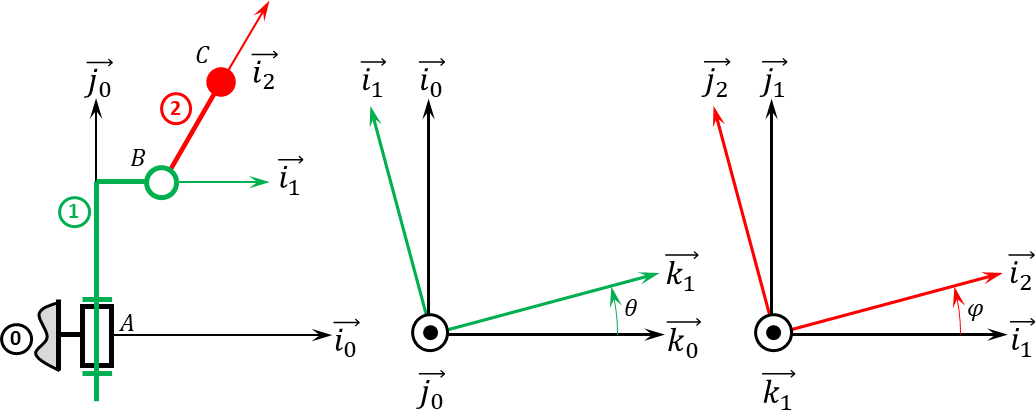
\includegraphics[width=\linewidth]{08_RR3D_01}
\end{marginfigure}
\fi

\question{Tracer le graphe des liaisons.}
\ifprof
\else
\fi

\question{Retracer le schéma cinématique en 3D pour $\theta(t)=\pi\,\text{rad}$ et $\varphi(t)=-\dfrac{\pi}{4}\, \text{rad}$.}
\ifprof
\else
\fi





\ifprof
\else

\marginnote{Corrigé  voir \ref{CIN:01:B2:12:08}.}

\fi